\documentclass{article}
\usepackage[T1,T2A]{fontenc}
\usepackage[utf8]{inputenc}
\usepackage[english,ukrainian]{babel}
\usepackage[]{amsthm} %lets us use \begin{proof}
\usepackage[]{amssymb} %gives us the character \varnothing
\usepackage{graphicx}

\begin{document}

\title{Семінар 16. Алгоритми Прима і Крускала}
\date{27 червня 2023}

\maketitle

\subsection*{Згадаємо означення}
Зв'язаний граф, дерево, кістякове дерево

\subsection*{Алгоритм Крускала}
\begin{itemize}
    \item Проініціалізувати граф T з усіма вершинами але без ребер
    \item Відсортувати ребра (яка складність?)
    \item Ітеруючись по відсортованим ребрам:
        \subitem якщо ребро не утворює цикл в T - додати його в T
    \item T - мінімальне кістякове дерево
\end{itemize}

\begin{figure}[h]
\centering
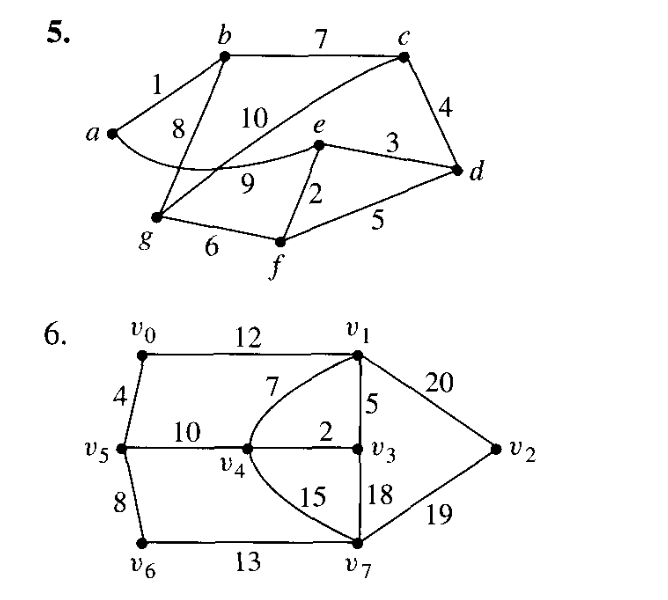
\includegraphics[width=90mm]{1}
\end{figure}

\subsection*{Система неперетинних множин (СНМ)}
Система неперетинних множин - це структура данних, яка відстежує розбиття множини на підмножини, вона вміє за "константний" час
\begin{itemize}
    \item Додавати новий елемент (і записати в нову підмножину)
    \item Об'єднати дві підмножини
    \item Повернути підмножину в якій знаходиться елемент
\end{itemize}

\begin{figure}[h]
\centering
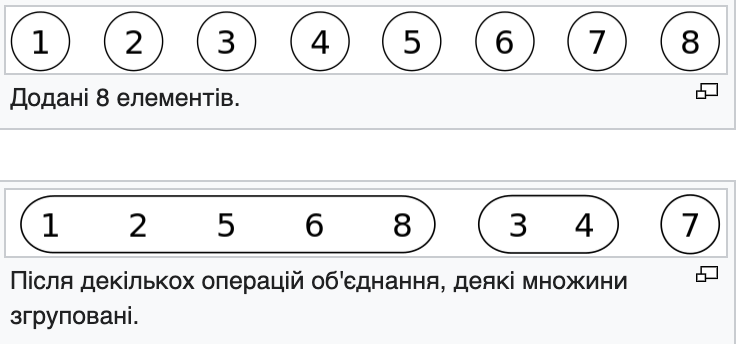
\includegraphics[width=90mm]{2}
\end{figure}

\subsection*{Алгоритм Крускала v2}
\begin{itemize}
    \item Проініціалізувати СНМ з усіма вершинами
    \item Відсортувати ребра
    \item Ітеруючись по відсортованим ребрам:
        \subitem якщо ребро зв'язує дві різні множини - додати його, множини об'єднати
        \subitem якщо додали n-1 ребро - закінчити (міні оптимізація)
\end{itemize}

\begin{figure}[h]
\centering
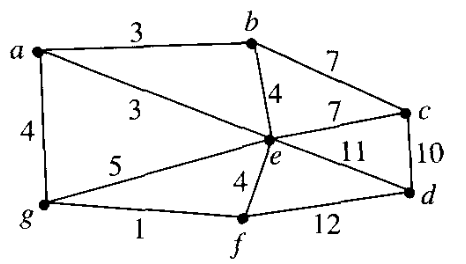
\includegraphics[width=90mm]{3}
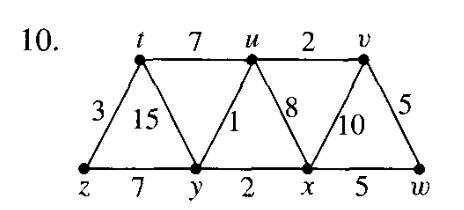
\includegraphics[width=90mm]{4}
\end{figure}

\pagebreak

\subsection*{Алгоритм Прима}
\begin{itemize}
    \item Обрати довільну вершину v, T - граф тільки з вершиною v, V - множина вершин без v
    \item Ітеруючись від 1 до n-1:
        \subitem обрати найменше ребро e, що з'єднує T з якоюсь вершиною V - w
        \subitem додати e, w у граф T; w прибрати з V
\end{itemize}

\begin{figure}[h]
\centering
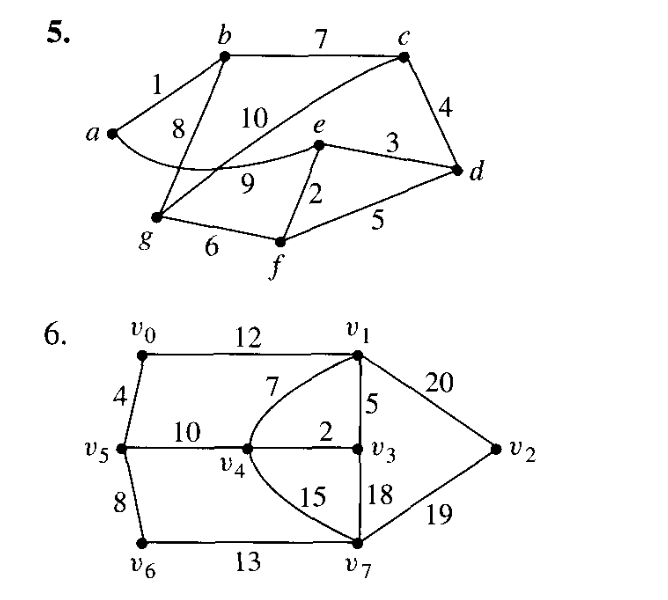
\includegraphics[width=90mm]{1}
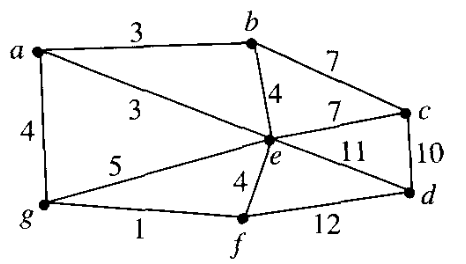
\includegraphics[width=90mm]{3}
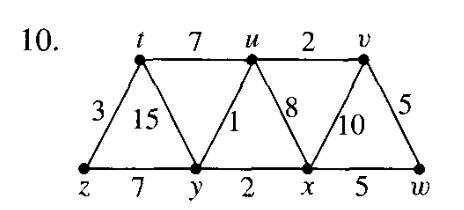
\includegraphics[width=90mm]{4}
\end{figure}

\end{document}